\documentclass[letterpaper, 10pt, conference]{ieeeconf}  % 
\IEEEoverridecommandlockouts                              % This command is only needed if 
                                                          % you want to use the \thanks command
\overrideIEEEmargins    
\usepackage{cite}

\usepackage{algorithmic}

\usepackage{textcomp}

\usepackage{comment}

%\usepackage{graphicx}      % include this line if your document contains figures
%\usepackage{natbib}        % required for bibliography
%===============================================================================
% Needed to meet printer requirements.
 \usepackage{latexsym,amssymb,amsfonts}
\usepackage[applemac]{inputenc}
\usepackage{rotating}
\usepackage{cite}
%\usepackage{graphicx}
\usepackage{epstopdf}
\usepackage{subfigure}
%\usepackage{color}
%\usepackage{xcolor}
%
%\usepackage{color}
\usepackage[dvipsnames]{xcolor}
%
\usepackage[normalem]{ulem}
\usepackage{isolatin1}
%\usepackage{caption}
%\usepackage{array,multirow,makecell}
%\usepackage{placeins}
%\usepackage{stackengine}
%\usepackage{hyperref}
\usepackage{fancybox}
\usepackage{colortbl}
\usepackage{float}
\usepackage{comment}
\usepackage{mathdots}
%\usepackage{lmodern}
%%%%%%%%%%%%%%%%%%%%%%%%%%%%%%%%%%%%%%%%%%%%%%%%%%%%%%%%%
\usepackage{dblfloatfix}
\usepackage{kantlipsum}
\usepackage{dblfloatfix}    % To enable figures at the bottom of page
\usepackage{graphicx} % [demo] option for empty figure
\usepackage{placeins}
\usepackage{marginnote}
\usepackage{url}
\usepackage{hyperref}
\usepackage{fancybox}
%\usepackage{empheq}
\usepackage[overload]{empheq}

\usepackage{bm}

%%%%%%%%%%%%%%%%%%%%%%%%%%%%%%%%%%%%%%%%%%%%%%%%%%%%%%%%%
\usepackage{tikz}
\usetikzlibrary{circuits.ee.IEC}
\usepackage[european resistor, european voltage, european current]{circuitikz}
\usetikzlibrary{arrows,shapes,positioning}
\usetikzlibrary{decorations.markings,decorations.pathmorphing,
decorations.pathreplacing}
\usetikzlibrary{calc,patterns,shapes.geometric}
\usetikzlibrary{shapes.multipart,positioning,patterns,backgrounds}
\tikzstyle{titlebox}=[rectangle,inner sep=10pt,inner ysep=10pt,draw]%

%%%%%%%%%%%%%%%%%%%%%%%%%%%%%%%%%%%%%%%%%%%%%%%%%%%%%%%%%%%%%

\def\blacksquare{\hbox{\vrule width 4pt height 4pt depth 0pt}}
\def\square{\hbox{\vrule\barox{\hrule\phantom{o}\hrule}\vrule}}
\def\qed{\hfill \square}
\def\qedp{\rightline{$\blacksquare$}}
\def\EXPT{\mathop{{\rm E}}}
\def\MIN{\mathop{{\rm min}}}
\def\MAX{\mathop{{\rm max}}}
\def\LIM{\mathop{{\longrightarrow}}}
\def\UNION{\mathop{\bigcup}}
\def\INTERSECT{\mathop{\bigcap}}
\def\ARGMIN{\mathop{{\rm argmin}}}
\def\ARGMAX{\mathop{{\rm argmax}}}
\def\TOUND{\mathop{\longrightarrow}}
\def\col#1{\mathop{{\rm col}\,\left(\,#1\,\right)}}
\def\eqref#1{(\ref{#1})}
\def\rank{\mathop{{\rm rank}}}

\newcommand{\widebox}[2][0.5em]{\fbox{\hspace{#1}$\displaystyle #2$\hspace{#1}}}


%\newcommand*\rank{\rm rank}
\def\rank{\mathop{{\rm rank}}}

%%%
\newtheorem{prb}{\it Problem}%[section]
\newtheorem{theorem}{\it Theorem}%[section]
\newtheorem{lemma}{\it Lemma}%[section]
\newtheorem{definition}{\it Definition}
\newtheorem{remark}{\it Remark}%[section]
\newtheorem{assumption}{\it Assumption}%[section]
\newtheorem{example}{\it Example}%[section]b
\newtheorem{annex}{\it Annex}%[section]b
\newtheorem{prop}{\it Proposition}%[section]b








\def\BibTeX{{\rm B\kern-.05em{\sc i\kern-.025em b}\kern-.08em
    T\kern-.1667em\lower.7ex\hbox{E}\kern-.125emX}}

\begin{document}


\title{\bf Resilience in Distributed
 Consensus based on Trust for Conneted Vehicle }
\author{Q.H. Nguyen$^{1,2}$, Shengya Meng $^{1}$, H. Rafaralahy $^{1}$, M. Haddad $^{2}$, A. Zemouche $^{1}$
%
\thanks{This work was supported by SEGULA Engineering. H. Rafaralahy and A. Zemouche would like to acknowledge the ANR agency for its partial financial support under the project ArtISMo ANR-20-CE48-0015.
}
%
\thanks{$^{1}$ Universit\'e de Lorraine, CRAN  CNRS UMR 7039, 54400 Cosnes et Romain, France~(e-mail: \protect\url{ali.zemouche@univ-lorraine.fr}).}
%
\thanks{$^{2}$ SEGULA Engineering, 19 rue d'Arras, 92000 Nanterre, France~(e-mail: \protect\url{madjid.haddad@segula.fr}).}
%
\thanks{All relevant CARLA resources have been made available in \protect\href{https://github.com/kslhuy/CACC_UIO_simulink}{GitHub}.}
}
\maketitle

\begin{abstract}

 To address this problem, we pro
pose a distributed driving state observer inspired by the leader-follower consensus technique. This observer can reconstruct the global driving state of the platoon, including the positions, velocities, and accelerations of all vehicles. We also derive the necessary and sufficient conditions to ensure the stability of its estimation error dynamics.
This work considers the problem of resilient consensus, where stochastic values of trust between agents are available. Specifically, we derive a unified mathematical framework to characterize convergence, deviation of the consensus from the true consensus value, and expected convergence rate, when there exists additional information of trust between vehicles.We show that under certain conditions on the stochastic trust values and consensus protocol: First, almost sure convergence to a common limit value is
possible even when malicious agents constitute more than half of the network connectivity; second, the deviation of the converged limit,
from the case where there is no attack,i.e.,the true consensus value.
\end{abstract}

\begin{keywords}
Distributed observers, secure estimation, lyapunov stability, cyber-attack.
\end{keywords}

\section{Introduction}

 The objective of global driving state
 estimation is to design an estimation algorithm for each vehicle
 to determine the positions, velocities, and accelerations of all
 vehicles in the platoon using only locally available information

 As a platoon is a typical networked control system (NCS),
 there has been a recent surge of interest in distributed driving
 state estimation

    
Contributions in the Context of Previous Work: This article builds most closely off of our previous work in [20] and[55], which shows that a stochastic variable $\alpha_{ij}(t)$ can be extracted
 from wireless signals between agents to verify the validity of an
 agent's identity (in a probabilistic sense) during a Sybil attack.
 Furthermore, Gil et al. [55], [56] show the potential of using
 these values to arrive at resilient consensus. In the current work,
 we assume the availability of such probabilistic observations of
 trust between agents, $\alpha_{ij}(t)$, and focus on the development of the
 mathematical machinery that can utilize these trust values to ar
rive at strong results for resilient consensus. Key differentiating
 results include the following.
 1) We provide convergence rate results for the case where
 the number of malicious agents is larger than 1/2 of the
 network connectivity, showing that convergence in finite
 time is possible with arbitrarily high probability. To the
 best of our knowledge, this is the first time that this result
 has been formally proven.
 2) We divide the consensus algorithm into two critical stages with broad consequences for the attainable performance guarantees. In the first stage, the agents observe the net
work, i.e., they collect values of $\alpha_{ij}(t)$ to detect malicious agents but do not start running the consensus protocol.
 In the second stage, agents continue to collect values of
 $\alpha_{ij}(t)$ and also adapt their data values using a modified consensus protocol that includes received data only from agents they classify as trustworthy. We show that the
 impact of observing the network for some time window T0 is highly consequential for deviation and convergence,
 where convergence rate and deviation amount decreases
 exponentially with increasing T0.
 3) We use weights that define a switching topology allowing for arbitrarily small deviation in the final consensus value.
 4) The current work allows for the use of nonsymmetric weights, which can accommodate larger classes of multiagent systems.
 Finally, the results in this article are general to many classes
 of attacks so long as certain characteristics on the probability
 of trust between agents, $\alpha_{ij}(t)$, are met. We establish these key
 characteristics and define their roles in convergence, deviation,
 and convergence rate to consensus.
The contributions of this paper are as follows:
\begin{enumerate}
\item Trust to opinion
\item Trust to controller
\item Trust to observer

\end{enumerate}


\section{Graph Representation}
Let $G = (V, E)$ be an undirected graph with $n$ nodes, where:
\begin{itemize}
    \item $V = \{1, 2, \dots, n\}$ is the set of nodes.
    \item $E \subseteq V \times V$ is the set of edges.
    \item The adjacency matrix $A$ of the graph $G$ is an $n \times n$ matrix where:
\end{itemize}
\begin{equation}
        A_{ij} = \begin{cases}
            1, & \text{if node } i \text{ connect} \text{ to node } j , \\
            0, & \text{otherwise}.
        \end{cases}
    \end{equation}
\subsection{Virtual Graph Generation}
For each vehicle $j \in \{1, 2, \dots, n\}$, we generate a virtual graph $G^{(j)} = (V^{(j)}, E^{(j)})$ by adding an extra node $0$ and connecting it to node $j$ and its neighbors.

\begin{itemize}
    \item The set of nodes in the virtual graph $G^{(j)}$ is $V^{(j)} = \{0\} \cup V$.
    \item  The set of edges in the virtual graph $G^{(j)}$ is $E^{(j)} = E \cup \{(0, j)\} \cup \{(0, k) \mid k \in \text{neighbors of } j$
    \item The adjacency matrix $V^{(j)}$ of the virtual graph $G^{(j)}$ is an $(n+1) \times (n+1)$ matrix defined as:
    \begin{equation}
        V^{(j)} = \begin{bmatrix} 0 & \mathbf{v}_j^T \\ \mathbf{v}_j & A \end{bmatrix}
    \end{equation}
    where $\mathbf{v}_j$ is a column vector of size $n$ such that:
    \begin{equation}
        \mathbf{v}_j(i) = \begin{cases}
            1, & \text{if } i = j \text{ or } A_{ji} = 1, \\
            0, & \text{otherwise}.
        \end{cases}
    \end{equation}
    This means that node $0$ is connected to node $j$ and all its neighbors in the original graph.
\end{itemize}

% \subsection{Consensus Weights Calculation}
% For each virtual graph $G^{(j)}$, we calculate the consensus weight matrix $W^{(j)}$. The weight matrix $W^{(j)}$ is an $(n+1) \times (n+1)$ matrix where $W^{(j)}(i, l)$ represents the weight assigned to the edge between node $i$ and node $l$.

% The degree $d_i$ of node $i$ in $G^{(j)}$ is given by:
% \begin{equation}
%     d_i = \sum_{l=1}^{n+1} V_j(i, l)
% \end{equation}

% The weight matrix $W^{(j)}$ is then defined as:
% \begin{equation}
%     W_{i, l}^{(j)} = \begin{cases}
%         \frac{1}{d_i + 1}, & \text{if } V_j(i, l) = 1 \text{ or } i = l, \\
%         0, & \text{otherwise}.
%     \end{cases}
% \end{equation}

% This means that the weight $W_{i, l}^{(j)}$ is $\frac{1}{d_i + 1}$ if there is an edge between node $i$ and node $l$ or if $i = l$ (self-loop), and $0$ otherwise.

% \subsection{Summary}
% \begin{itemize}
%     \item \textbf{Virtual Graph $G_j$:} For each vehicle $j$, the virtual graph $G_j$ is constructed by adding node $0$ and connecting it to node $j$ and its neighbors.
%     \item \textbf{Weight Matrix $W_j$:} The weight matrix $W_j$ is calculated based on the degree of each node in the virtual graph $G_j$.
% \end{itemize}

% \subsection{General Form}
% For a general graph $G = (V, E)$ with adjacency matrix $A$, the virtual graph $G_j$ and its corresponding weight matrix $W_j$ can be expressed as:
% \begin{equation}
% \begin{aligned}
%     G_j = (V_j, E_j), \quad V_j = \{0\} \cup V, \\ E_j = E \cup \{(0, j)\} \cup \{(0, k) \mid k \in \text{neighbors of } j\}    
% \end{aligned}
% \end{equation}

% \begin{equation}
%     W_j(i, l) = \begin{cases}
%         \frac{1}{d_i + 1}, & \text{if } (i, l) \in E_j \text{ or } i = l, \\
%         0, & \text{otherwise}.
%     \end{cases}
% \end{equation}


\section{General description}\label{sec:genral}
\subsection{Local System}
The Minicar has Ackermann steering geometry, and its kinematics can be approximated by the bicycle model, with motion equations as follows:
where
\begin{align} \label{diff_1_LPV}
    \dot{X} &= v cos(\theta) \\ \notag
    \dot{Y} &= v sin(\theta)\\ \notag
    \dot{v} &= a \\ \notag
    \dot{\theta} &= L^{-1} v tan(\delta)  \\
    or \quad
    \dot{\theta} &= \omega  
\end{align}
\begin{itemize}
    \item $X , Y$ denote the position,
    \item v is is the forward speed , a acceleration control 
    \item $\delta $ is the steering angle,
    \item L is the vehicle's wheel base. 
\end{itemize}

Each vehicle has a full measurement state obtained in real-time \textbf{position} and \textbf{velocity}, \textbf{heading angle} from a GPS, IMU sensor mounted on the vehicle. 

The radar sensor is located on the front of the
 host vehicle and measures the relative speed and distance to the rear bumper of the target
 vehicle. The relative distance $r$ is defined as

\begin{equation}\label{radar}
    r = \sqrt{(X_t - X_h)^2 + (Y_t - Y_h)^2} - L 
\end{equation}
$X$ and $Y$ positions of the host and preceding vehicle vehicle
 correspond with their center of gravity. Note that the expression in \eqref{radar} is a simplification
 where the difference in heading angle between the two vehicles is ignored. The effects of
 this simplification can be included in the measurement noise, which also accounts for the
 $r$ is defined as uncertainty of the measurement location on the target vehicle's bumper. The relative speed $\dot{r}$
 \begin{equation}\label{radar_speed}
     \dot{r} = (v_t - v_h) cos(\theta_r)
 \end{equation}
where $r$ is the azimuth angle measured by the radar. The relative speed is derived from a
 constant radius cornering assumption where the vehicles drive with the same curvature
 and have no relative lateral offset with respect to the desired trajectory.

%  \textcolor{red}{The dynamics of $i^{th}$ vehicle are a Position-Velocity third-order linear model given by the following set of equations:}

% \begin{equation}\label{eq_1}
%       \left\{ \begin{array}{l}
%         \dot{p}_i(t) =v_i(t) \\
%         \dot{v}_i(t) =a_i(t)  \\
%         \end{array}  \right.
% \end{equation}  
% where
% \begin{itemize}
% \item $p_i(t), v_i(t)$ and $a_i(t)$ denote the position, velocity and
% acceleration of the $i^{th}$  vehicle, respectively;
% \item $u_i(t)$ is the $i^{th}$ vehicle control input representing the desired
% driving/braking force or acceleration;
%  \item $\tau$ is the engine's constant time lag. 
 
%  \end{itemize}

%  All the equations can written :

% \begin{equation}\label{CACC}
% %\displaystyle
%        \begin{array}{l}
%         {x_i}(t+1)=A x_i + B  u_i + B_f f(x)_i  \\
%         y_{i}(t) = Cx_{i}\end{array} .
% \end{equation}  

% where 
% \begin{equation*}
%         A  =\begin{bmatrix}
%         0 & 1 & 0 \\
%         0 & 0 & 1 \\
%         0 & 0 & \frac{-1}{\tau}
%           \end{bmatrix},
%         B =\begin{bmatrix}
%         0 \\
%         0 \\
%         \frac{1}{\tau}
%           \end{bmatrix}, 
%         B_f =\begin{bmatrix}
%         0,0 \\
%         1,0 \\
%         0,1
%           \end{bmatrix},
%         C =\begin{bmatrix}
%         1 & 0 & 0 \\
%         0 & 1 & 0 \\
%         0 & 0 & 1
%           \end{bmatrix}, 
% \end{equation*}





\subsection{Model Discretization}
 In order to adopt a state-space notation , a cascading system description is considered, allowing us to transform the system
 dynamics into state-space form. The schematics of the cascading systems approach is
 shown in Figure \ref{fig:2sys},

\begin{figure}[htp]
    \centering
    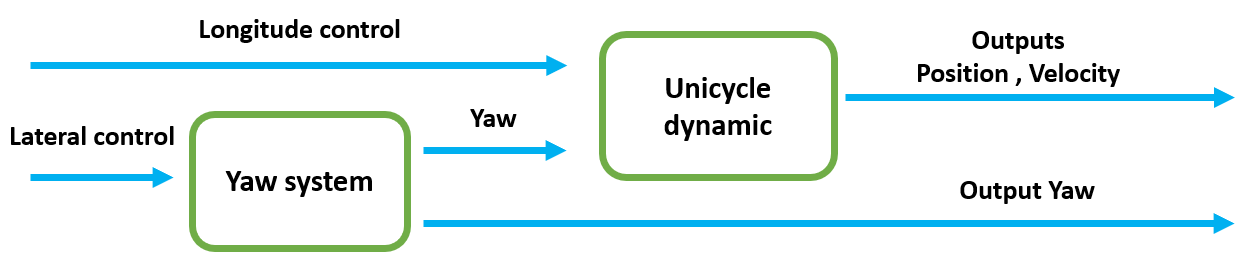
\includegraphics[scale=0.4]{img/2system.png}
    \caption{Schematic of the cascading systems.}
    \label{fig:2sys}
\end{figure}

$$
\begin{gathered}
\mathbf{x}_1=\left[\begin{array}{ll}
  \theta_{\mathrm{h}} & \dot{\theta}_{\mathrm{h}}
\end{array}\right]^T \\
\mathbf{x}_2=\left[\begin{array}{lll}
 X_{\mathrm{h}} & Y_{\mathrm{h}} & v_{\mathrm{h}}
\end{array}\right]^T
\end{gathered}
$$

measurement vectors

$$
\begin{array}{c}
\mathbf{y}_1=\left[\begin{array}{ll}
 \theta_{\mathrm{h}} & \dot{\theta}_{\mathrm{h}}
\end{array}\right]^T \\
\mathbf{y}_2=\left[\begin{array}{lllll}
 X_{\mathrm{h}} & Y_{\mathrm{h}} & v_{\mathrm{h}} & \dot{\theta}_{\mathrm{h}} & r
\end{array} \right]^T \\
\end{array}
$$

and process noise vectors



are introduced. In state-space form, the system dynamics are described as

$$
\begin{aligned}
\dot{\mathbf{x}}_j=\mathbf{A}_j \mathbf{x}_j+\mathbf{B}_j \mathbf{u}_j+\mathbf{E}_j \mathbf{w}_j, \\
\mathbf{y}_j=\mathbf{C}_j \mathbf{x}_j+\mathbf{D}_j \mathbf{u}_j+\mathbf{J}_j \mathbf{v}_j,
\end{aligned}
$$

   
\subsection{Distributed/Collective system}


So we can write down the the virtual global system that represents all the k-neighbors of $i^th$ . 



\begin{equation}\label{CACC_dis_neibor}
        \mathbf{{X}}(t+1)=\mathbf{A} \mathbf{X} + \mathbf{B}({U + \mathcal{D}_{uk}}) 
\end{equation}

where 
\begin{equation*}
\mathbf{A} = I_N \otimes A_i, \quad \mathbf{B} = I_N \otimes B_i,
\end{equation*}




So the 

\begin{itemize}
\item $\mathbf{X} = [x_{i-k},..., x_{i} ,..., x_{i+k}]^T$ 
\item $U = [u_i , ... u_i ,.. u_i ]^T$ 


 \item $\mathcal{D}_{uk}$ is the uncertain in the controller input. 
 \end{itemize}


The Global System's state can be categorized into lead, follower, and last positions.


\section{ System Architecture and Design of controller}

\begin{figure}[htp]
    \centering
    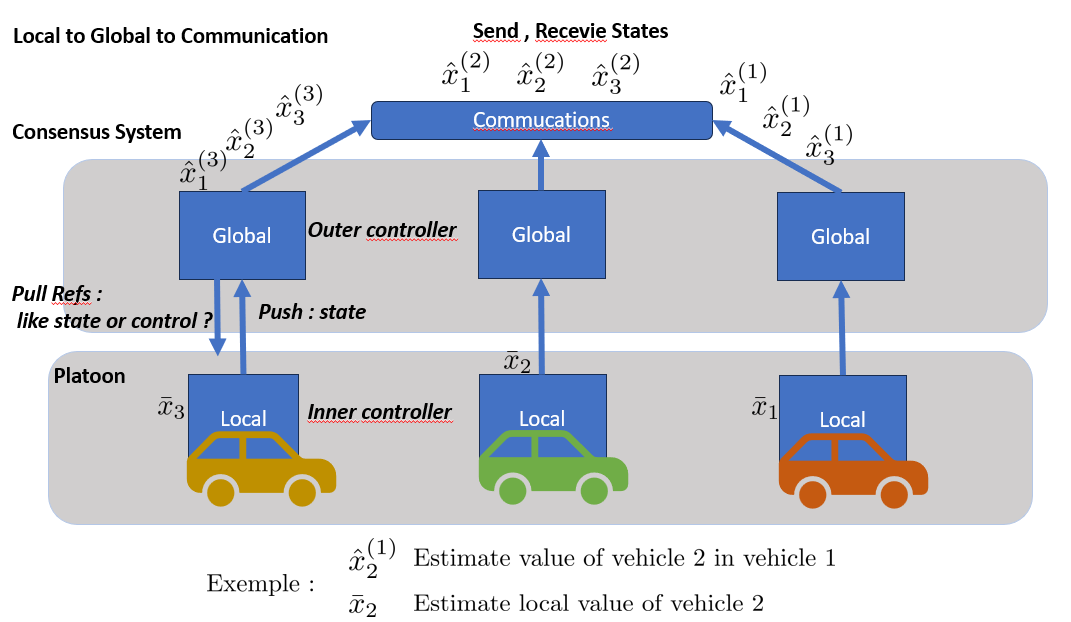
\includegraphics[scale=0.45]{img/local_global_com.png}
    \caption{Schematic diagram of the estimation method.}
    \label{fig:information_boarcard}
\end{figure}

We will have two controllers: the inner controller (local control) and the outer controller (distributed control), located in the internal and external control loops of the vehicle, respectively. The inner controller is responsible for ensuring that the vehicle follows its reference trajectory while maintaining a safe distance from the preceding vehicle; this is commonly referred to as the Adaptive Cruise Control (ACC) controller. The outer controller, which we will refer to in this paper as the Distributed Observer Cooperative Adaptive Cruise Control (CACC), is designed to facilitate consensus within a platoon of vehicles. The CACC aims to minimize the distance between vehicles in a platoon so that the group can travel more quickly and smoothly. These 2 controllers will be combined to get the final controller to actually put in the control loop. 
\ref{fig:information_boarcard}



\subsection{Inner / Local controller}
 The local system on longitudinal motion by using Intelligent Driver Model (IDM) was first proposed in $[..]$.
 The idea under-pinning IDM is that a vehicle's acceleration is a function of the vehicle's current velocity v, it's gap s
 to the preceding vehicle, and the approach rate $\Delta v$ to the preceding vehicle. It is formalized as :
 \begin{equation}
    a_{\mathrm{IDM}}=\alpha\left[1-\left(\frac{v}{v_0}\right)^\delta-\left(\frac{s^{\star}(v, \Delta v)}{s}\right)^2\right]
 \end{equation}

where $s^{\star}$ is a function determining the desired minimum gap to the preceding vehicle. We compute this value as

\begin{equation}
s^{\star}(v, \Delta v)=s_0+T v+\frac{v \Delta v}{2 \sqrt{\alpha \beta}}.    
\end{equation}

where $s_0$ corresponds to a jam distance. 

\subsection{Cooperative controller}
Nevertheless, the classical IDM that only considers the impacts of the nearest preceding vehicle is insufficient to describe the CAV
behaviors, where each CAV exchanges information with multiple surrounding vehicles. Hence, a revised IDM incorporating cooperation through wireless communications, labeled cooperative IDM (CIDM) \cite{C_IDM}, is formulated by the following equations:
\begin{equation}\label{CIDM}
a_{CIDM}=\alpha \left[1-\left(\frac{v_n(t)}{v_0}\right)^4-\left(\frac{S^{*}\left(v_n(t), \Delta \tilde{v}_{n-j+1}(t)\right)}{\sum_{j=1}^N \alpha_{n j} w_{n j} \tilde{{s}}_{n-j+1}(t)}\right)^2\right] 
\end{equation}
with
\begin{equation*}
\begin{aligned}
    S^{*}\left(v_n(t), \Delta \widetilde{v}_{n-j+1}(t)\right)=s_0+T v_n(t)+ \\ \frac{v_n(t) \cdot \sum_{j=1}^N \beta_{n j} w_{n j} \Delta \tilde{v}_{n-j+1}(t)}{2 \sqrt{a b}} .
\end{aligned}
\end{equation*}

In the steady-state, all vehicles travel at the same velocity $\nu^{\text {eq }}$ with the same clearance gap $s^{\text {eq }}$. Eq. \eqref{CIDM} yields the uniform clearance gap as follows:

\begin{equation}\label{gap_CIDM}    
s^{\mathrm{eq}}(v)=\left(s_0+T v^{\mathrm{eq}}\right)\left(1-\left(\frac{v^{\mathrm{eq}}}{v_0}\right)^4\right)^{-1 / 2}
\end{equation}
Eq. \eqref{gap_CIDM} shows that each following vehicle's gap at equilibrium is determined by the equilibrium velocity. However, once an
attack occurs, the equilibrium clearance gap and velocity will be perturbed.

\subsection{Final Controller}
The control to the vehicle is 
\begin{equation}
    u_{tot} = \gamma. a_{IDM} + (1-\gamma).a_{CIDM} 
\end{equation}
where, the parameter $\gamma$ is used for tuning the control strategy, can be determined by the level of trust we have in the connection.. It allows us to combine two types of control for optimal performance. When $\gamma = 0$, we rely entirely on cooperative control, which is beneficial when we have a strong connection. Conversely, when $\gamma = 1$, we use the Intelligent Driver Model (IDM) solely based on local sensor data to drive the controller. The vehicle's control input at time $t$ is computed through the integrator $v_t= u _{\mathrm{tot}}$. $\Delta t + v_{t-1}$.

%% ------------------------------------

\section{Distributed Driving State Estimation Scheme}
Similarly to controller, the estimation step also has 2 distinct designs. 
\subsection{Local Observer Design}
\begin{equation}\label{observer_dis_plug}
\bar{x}_i(k+1)=A \bar{x}_1(k)+B u_1(k)+F_1(y_1(k)-C \bar{x}_1(k))
\end{equation}
The estimation error is : 
\begin{equation}
e_0^{(j)}(k+1)= A - F_j C
\end{equation}
The main goal is to find the appropriate values for the observer gains $F_j$ by solving certain LMIs [..] or Kalma filter. This is done in order to ensure that the estimation error $e_0^{(j)}$ converges to zero asymptotic. 

\begin{remark}
In a local observer, we have the flexibility to develop a better model for improved estimation results, such as using model [...]. The idea is that a local observer will consistently provide accurate estimates, while remaining decoupled from the distributed observer.
\end{remark}

\subsection{Distributed Observer Design}
In this section, we focus on a collective layer system in which each vehicle can estimate the platoon's stats, so we call this distributed observer. We develop a distributed driving state observer for a vehicle platoon and establish conditions that guarantee
the stability of its estimation error dynamics.



This distributed state estimation \textcolor{blue}{like shenya paper} procedure can be summarized as follows :

\begin{equation}
\dot{\hat{X}}_i=A \hat{X}_i+F+L_i\left(\bar{C}_i \hat{X}_i-\bar{y}_i\right)+r_i P_i^{-1} \sum_{j=1}^N a_{i j}\left(\hat{X}_j-\hat{X}_i\right),
\end{equation}

\ref{Weigth_Design}. 

\remark{It is difficult to get, or send the control input because it will be private. So we will consider that all the controllers in vehicle $k^{th}$ that is the neighbor of $i^{th}$ vehicle will be  $u_k = u_i + d_{u_k}$ , $d_{u_k}$ is a bound have a bound value. so the controller in the virtual global system  $U = [u_{1} , u_2 ,.. u_{j} ]^T$ }

\textbf{Explain the concept of an observer:} The system aims to get all states of the platoon, so the second term focuses on improving the global estimate in each vehicle by compensating with communication data. However, since the initial global state of the platoon in each vehicle is incorrect and we do not have precise information about the controllers, nor good models of other vehicles for accurate predictions, we address this uncertainty with the third term and use local estimation as a ref to achieve. The first term is then combined with the other terms to predict the overall global state of the system in the next step.

% \textbf{Explain the concept of an observer:} The system aims to reach a consensus value, so the second term focuses on improving the global estimate in each vehicle by compensating with communication data. However, since the initial global state of the platoon in each vehicle is incorrect and we do not have precise information about the controllers of other vehicles for accurate predictions, we address this uncertainty with the third term, which attempts to achieve a local estimation of these others. The first term is then combined with the other terms to predict the overall global state of the system in the next step.


\remark{Note that the information transmitted
by each vehicle $i \in V$ through the communication network $G$ is
the local estimate and the global estimate state of the platoon from each vehicle, i.e., $\hat{x}_i(k)$ and $\bar{x}_i(k)$.}

% \remark{k-neighbor of $i^th$ will send the local estimated value $\hat{x}_k $ to the $i^th$ vehicle and, also send about global estimated of all vehicles in the platoon.
% }

\section{Modeling Trust}


To prevent collisions induced by data injection attacks as demonstrated in \cite{C_IDM}, only accurate data can be passed to the cruise controller. Since a host vehicle cannot judge the value of a single data point received in a beacon, it has to be compared to the sender's actual behavior over a longer period of time. This allows the host vehicle to gain trust in the sender's benignity or detect misbehavior. Depending on the trust in the predecessor within the platoon, the host vehicle can regulate the safety gap to that vehicle. If the trust falls below a certain threshold, it might ultimately decide not to be in a platoon with that vehicle at all. This section introduces the details of TriP, our trust-based misbehavior detection system for platoons.

\assumption{In the virtual global system, there naturally aren't faults; the faults are caused by uncertainties or cyber-attacks in the communication channels.}

\subsection{Interactions}

A host vehicle with automated driving functions, such as Cooperative Adaptive Cruise Control (CACC), must ultimately trust its own sensor data. When assessing other platoon member's trustworthiness, the host vehicle uses its sensor data as ground truth to compare the others actual behavior to what they announced in their beacons. This comparison is feasible only for vehicles within the perception range of the host vehicle's local sensors and is most effective for the direct predecessor and successor. Inspire of \cite{trust_simple, trust_complex} each criterion evaluation results in a value between 0 (worst) and 1 (best). 

\paragraph{Velocity} The host vehicle calculates the reference velocity $v_\text{ref}$ based on the leader's last reported velocity $v_L$, adjusted by the reported acceleration $a_L$ and the elapsed time $b_L$ since the last leader beacon:
\begin{equation}
    v_\text{ref} = v_L + b_L \cdot a_L.
\end{equation}

\begin{itemize}
    \item Target Mismatch with the Leader
        \begin{equation}
        v_{y,\text{ref}} = 
        \begin{cases} 
            \max\left(1 - \left|\frac{v_y - v_\text{ref}}{v_\text{ref}}\right|, 0\right), & \text{if } v_\text{ref} > 0, \\
            \max\left(1 - |v_y|, 0\right), & \text{otherwise}.
        \end{cases}
    \end{equation}
    \item Target Mismatch with the Host
        \begin{equation}
            v_{y,\text{host}} = 
            \begin{cases} 
                \max\left(1 - \left|\frac{v_y - v_\text{host}}{v_\text{host}}\right|, 0\right), & \text{if } v_\text{host} > 0, \\
                \max\left(1 - |v_y|, 0\right), & \text{otherwise}.
            \end{cases}
        \end{equation}
    % \item Host Mismatch with the Leader
    %     \begin{equation}
    %         v_{host,\text{leader}} = 
    %         \begin{cases} 
    %             \max\left(1 - \left|\frac{v_{host} - v_\text{ref}}{v_\text{ref}}\right|, 0\right), & \text{if } v_\text{ref} > 0, \\
    %             \max\left(1 - |v_y|, 0\right), & \text{otherwise}.
    %         \end{cases}
    %      \end{equation}
\end{itemize}
Fusion of these Mismatches using weighted average :
\begin{equation}
    v_{y,final} = \alpha. v_{y,leader} + (1-\alpha). v_{y,host}     
\end{equation}

The alpha will change depending on the position of the target vehicle. If the target is following the host, then alpha will ideally be around 0-0.3. If the target is ahead of the host, alpha will be around 0.7-1.

\paragraph{Distance} The host vehicle calculates the error between the measured distance $d$ from its sensors and the reported distance $d_{b,y}$ from the preceding vehicle:
\begin{equation}
    d_y = \max\left(1 - \left|d_{b,y} - d\right|, 0\right).
\end{equation}

\paragraph{Acceleration} The relative velocity $v_\text{rel}$ is derived as the rate of change in distance $d$ over the sample interval $t_s$. The acceleration criterion is:
\begin{equation}
    a_y = \max\left(1 - \left|\frac{v_\text{rel}}{t_s} \cdot a_\text{diff}\right|, 0\right),
\end{equation}
where $a_\text{diff}$ is the difference between the received and measured host acceleration. The term $\frac{v_\text{rel}}{t_s}$ scales the effect of acceleration mismatch based on how fast the vehicles are moving relative to each other.
Acceleration differences matter more if two vehicles are close together and moving at different speeds.
If they are farther apart or moving at the same speed, acceleration differences are less critical.
This prevents small acceleration mismatches from being overly penalized when relative motion is low.

% Why is the Equation Designed This Way?
% A. Measuring Acceleration Consistency
% The trust formula measures how much the reported acceleration deviates from the actual acceleration.
% If the difference is large, it means the vehicle is not reporting correct acceleration values, which could be due to:
% Malicious behavior (e.g., injecting false data).
% The larger the deviation, the more trust should decrease.
% B. Scaling the Trust Impact Based on Relative Motion
% The term scales the effect of acceleration mismatch based on how fast the vehicles are moving relative to each other.
% Acceleration differences matter more if two vehicles are close together and moving at different speeds.
% If they are farther apart or moving at the same speed, acceleration differences are less critical.
% This prevents small acceleration mismatches from being overly penalized when relative motion is low.

%------------Jerkiness
% \paragraph{Jerkiness:} The absolute jerk $j_{y,\text{abs}}$ is evaluated, with penalties applied only if it exceeds a threshold $j_\text{thres}$:
% \begin{equation}
%     j_y = \min\left(\frac{j_\text{thres}}{j_{y,\text{abs}}}, 1\right).
% \end{equation}

\paragraph{Beacon Delivery Timeout} If a member vehicle $y$ fails to send a beacon within the expected timeout, the timeout factor $t_y$ is set to 0, otherwise it is set to 1.

\subsection{Trust Samples}

All criteria are combined into a single trust sample $t_y$:
\begin{equation}
    t_y = t_{o,y} \cdot v^{w_v}_{y,\text{ref}} \cdot d^{w_d}_y \cdot a^{w_a}_y 
\end{equation}
% \begin{equation}
%     t_y = t_{o,y} \cdot v^{w_v}_{y,\text{ref}} \cdot d^{w_d}_y \cdot a^{w_a}_y \cdot j^{w_j}_y,
% \end{equation}
where $w_v, w_d, w_a, w_j$ are the respective weights for the criteria. So the maximal value of trust will be : 
$\max{t_y} \leq 1$

\subsection{Building Trust}
Since the resulting trust samples for interactions may change over time and a trust is build over repeated interactions, these values need to be aggregated in a way that allows historic evolution, judgment on reliability and
certainty. Thus, the aggregation can be represented in a probability distribution function (PDF) by using the framework
of Bayesian statistics.


Bayesian trust systems from literature are often based on the Beta Reputation System [21] which utilizes the beta PDF [15]. The Beta Reputation System is only able to express ratings in two outcomes, such as trusted and untrusted. The Dirichlet Reputation System [22] however
enables more fine granular ratings compared to the Beta Reputation System, as is is based on the Dirichlet PDF which is the generalization of the Beta PDF, supporting an arbitrary number of outcomes.


To describe the trustworthiness, k = 5 mutually exclusive, equidistant and ascending trust rating levels [01] are defined as \textit{untrustworthy, bad, acceptable, good } and \textit{excellent}.

When vehicle x calculates a $t_y \in [0, 1]$ for vehicle y, it is mapped to a $k$-dimensional vector $r_y^x$ where every element of the vector is 0 except the one for the respective trust rating level (which is set to 1). The vector $r_y^x$ can be interpreted as probability distribution with a single outcome, determined
by the trust sample. 

Multiple outcome vectors $r_y^x$ from x for y are then aggregated in the rating vector:
\begin{equation}
    R_y = (R_y(1), . . . , R_y(k))
\end{equation}


Trust samples are aggregated over time using a Bayesian approach. The aggregated rating vector $R_y$ accumulates past outcomes as follows:
\begin{equation}
    R_{y,(t+1)} = (1 - \lambda_y) \cdot R_{y,t} + r_{xy},
\end{equation}
where $\lambda_y$ is an aging factor depending on the trust score $\alpha$:
\begin{equation}
    \lambda_y = \alpha \cdot w_t.
\end{equation}

The probability distribution vector $S_y$ is computed using an a priori distribution vector $a$:
\begin{equation}
    S_y(i) = \frac{R_y(i) + C \cdot a(i)}{C + \sum_{j=1}^k R_y(j)}.
\end{equation}

The trust score $\alpha$ is then calculated as:
\begin{equation}
    \alpha = \sum_{i=1}^k \frac{i-1}{k-1} \cdot S_y(i).
\end{equation}

\textbf{Question : How to get the trust value of the other vehicle that we don't have direct measurement to compare , to build the Trust ?} 
Since vehicle front, and back of the vehicle i, we can evaluate the trust.
But for other vehicles (j's), we cannot have a trust score, but notice that other vehicle $(k)$ may have trust for these other vehicles $(j's)$, so they send us the trust score of them. By that we can combine all these trusts to one single value for each vehicle in the platoon. That trust score of $(k)$ we call opinion. So we can have the full trust score (just call for simple) can see in fig. \ref{fig:opinon_trust}
\begin{figure}[htp]
    \centering
    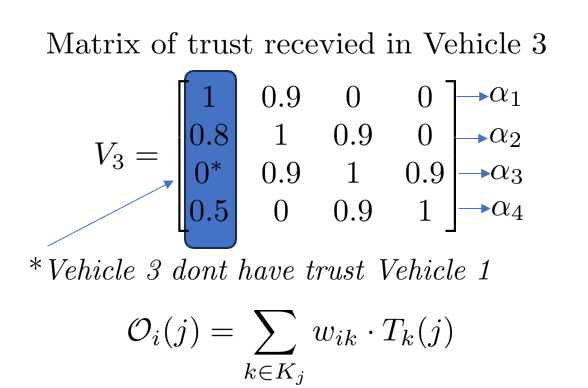
\includegraphics[scale=0.45]{img/opinon_trsut.png}
    \caption{New trust (Opinion). Trust Propagation Mechanism}
    \label{fig:opinon_trust}
\end{figure}


Product-Based Opinion Calculation
\begin{equation}
    \beta_i(j) = \prod_{k \in N_j} \alpha_k(j)
\end{equation}
\textcolor{red}{This Formule not good , change to weight-based sum}

Only calculate the opinion for the vehicle we don't have trust. 

\textcolor{red}{Big Question: We only use local to evaluate trust , how if the global being attack ? }

\textcolor{blue}{Answer: we need to check again the global ?, maybe not like local, but something like mean and variance ? . After that, by magic somehow can check the global, we could use that to change the weight, so that will related to parameter $\kappa$ in \eqref{kappa} }

\section{Weigth Design}\label{Weigth_Design}



\subsection{Introduction}
Prioritizing Directly Received Data in Trust Evaluation


When estimating the state of \textbf{vehicle 3} from the perspective of \textbf{vehicle 1}, the data received directly from vehicle 3 should carry more weight than the indirect opinions from intermediate vehicles (e.g., vehicle 2). This ensures that trust calculations prioritize the most relevant and up-to-date information. This document formalizes a weighting mechanism and dynamic adaptation strategy to achieve this.



\subsection{Weighting Trust Based on Data Proximity}
Instead of treating all received estimates equally, we introduce a weighting mechanism that prioritizes direct data over indirect reports.

\subsection{Weight Definition for Trust Calculation}
Let:
\begin{itemize}
    \item \( \alpha_{13} \) be the \textbf{direct trust} that vehicle 1 has in vehicle 3.
    \item \( \alpha_{23} \) be the trust that \textbf{vehicle 2} has in vehicle 3.
    \item \( \alpha_{12} \) be the trust that vehicle 1 has in vehicle 2 (used to evaluate indirect information).
\end{itemize}

The \textbf{final trust score for vehicle 3} from vehicle 1’s perspective is computed as:
\[
T_{1}(3) = w_1 \alpha_{13} + w_2 \sum_{k \in \mathcal{N}_1 \setminus \{3\}} w_k \alpha_{k3},
\]
where:
\begin{itemize}
    \item \( w_1 > w_k \) ensures that \textbf{direct trust is weighted more} than indirect trust.
    \item \( w_k \) is assigned based on vehicle 1’s trust in the intermediary vehicle \( k \).
\end{itemize}

\subsection{Weight Scaling Strategy}
To enforce a \textbf{higher priority on direct observations}, define:
\[
w_1 = 1 - \sum_{k \in \mathcal{N}_1 \setminus \{3\}} w_k
\]
and
\[
w_k = \frac{\alpha_{1k}}{\sum_{m \in \mathcal{N}_1 \setminus \{3\}} \alpha_{1m}} \cdot \gamma,
\]
where \( 0 < \gamma < 1 \) ensures indirect trust weights sum to a smaller portion.

\subsection{Example}
\begin{table}[h!]
\centering
\begin{tabular}{ccc}
\toprule
Vehicle & Trust in Vehicle 3 & Normalized Weight \( w_k \) \\
\midrule
Vehicle 1 (direct) & \( \alpha_{13} = 0.9 \) & 0.7 \\
Vehicle 2 (indirect) & \( \alpha_{23} = 0.8 \), \( \alpha_{12} = 0.6 \) & 0.3 \\
\bottomrule
\end{tabular}
\caption{Trust Weights for Direct and Indirect Data}
\end{table}

Here, \textbf{vehicle 1’s direct measurement of vehicle 3 dominates}, but \textbf{indirect opinions from vehicle 2} still contribute a small weight.



\subsection{Dynamic Adaptation of Weights}
The trust weighting should be \textbf{adaptive} based on \textbf{signal reliability} and \textbf{communication conditions}:
\begin{itemize}
    \item If \textbf{vehicle 1's direct estimate of vehicle 3 becomes unreliable} (e.g., sensor noise or packet loss), reduce \( w_1 \).
    \item If \textbf{vehicle 2 has a long history of reliable estimates}, increase \( w_2 \) proportionally.
\end{itemize}

The adaptive update rule is:
\[
w_1(t+1) = w_1(t) - \lambda \Delta R,
\]
where:
\begin{itemize}
    \item \( \lambda \) is a tuning parameter.
    \item \( \Delta R \) is the deviation between \textbf{vehicle 1's direct estimate} and the \textbf{averaged global estimate from others}.
\end{itemize}



\subsection{Implementation Steps}
\begin{enumerate}
    \item \textbf{Receive data} from vehicle 3 and intermediaries.
    \item \textbf{Compute direct trust \( \alpha_{13} \)} and indirect trust from other vehicles \( \alpha_{k3} \).
    \item \textbf{Assign higher weights to direct trust} using the weighting scheme.
    \item \textbf{Update weights dynamically} based on reliability metrics.
\end{enumerate}



By prioritizing directly received data and dynamically adapting trust weights, we ensure that trust evaluations are robust and reliable. This approach minimizes the influence of potentially compromised or unreliable indirect data sources.


\section{Estimation Error Dynamics}
In this part, we explore the conditions that guarantee the stability of the
estimation error dynamics of the proposed observer, as given in (5).

Using the error definitions:
\begin{align*}
e_0^{(j)}(k) = \bar{x}_i^{(j)}(k) - x_j(k),
\\
e_i^{(j)}(k) = \hat{x}_i^{(j)}(k) - x_j(k)
\end{align*}
The estimation error for the $j^{th}$ vehicle state as observed by vehicle $i$ is defined as:
\begin{align}
    e_i^{(j)}(k+1) = A[e_i^{(j)}(k) + \sum_{l \in \mathcal{N}_i} w_{il}^{(j)} (e_l^{(j)}(k) - e_i^{(j)}(k)) \notag \\
    + w_{i0}^{(j)}(e_0^{(j)}(k) - e_i^{(j)}(k))]. 
\end{align}
for the followers $( i, j \in V )$.

Let $e^{(j)}(k)=\left[e_0^{(j)}(k)^{\top}, e_1^{(j)}(k)^{\top}, \ldots, e_m^{(j)}(k)^{\top}\right]^{\top}$. Based on the error dynamics (8), we obtain the following composite error dynamics:
$e_i^{(j)}(k+1) = R^{(j)} e^{(j)}(k) $

The matrix $R^{(j)}$ describes how the estimation errors evolve within the network. It has the following block structure:

$$
R^{(j)}=\left[\begin{array}{cccc}
R_{00}^{(j)} & R_{01}^{(j)} & \cdots & R_{0 m}^{(j)} \\
R_{10}^{(j)} & R_{11}^{(j)} & \cdots & R_{1 m}^{(j)} \\
\vdots & \vdots & \ddots & \vdots \\
R_{m 0}^{(j)} & R_{m 1}^{(j)} & \cdots & R_{m m}^{(j)}
\end{array}\right]
$$

where:
\begin{itemize}
    \item  $R_{00}^{(j)}=A-F_j C_{j, j}$ : This block captures the error dynamics of the virtual node (vehicle $j$ 's own estimate).
    \item $R_{0 i}^{(j)}=0$ for $i \neq 0$ : The virtual node's error does not directly depend on other vehicles' errors.
    \item $R_{i 0}^{(j)}=A w_{i 0}^{(j)}:$ This block captures the influence of the virtual node's error on vehicle $i$ 's error.
    \item Let $\left(1-\sum_{l \in N_i} w_{i l}^{(j)}-w_{i 0}^{(j)}\right) = w_{i i}^{(j)}$ 
    , so $R_{i i}^{(j)}=A w_{i i}^{(j)}$ : This block captures the contribution of vehicle $i$ 's own error. 
    \item $R_{i l}^{(j)}=A w_{i l}^{(j)}$ for $l \in N_i$ : This block captures the influence of neighboring vehicles' errors vehicle $i$ 's error.
\end{itemize}

Or we can write compact form : 
$$
\begin{aligned}
e^{(j)}(k+1)= & \underbrace{\left[\begin{array}{c|c}
A-F_j C_{j, j} & \mathbf{0} \\
\hline O^{(j)} \otimes A & Q^{(j)} \otimes A
\end{array}\right]}_{R^{(j)}} e^{(j)}(k) 
\end{aligned}
$$
The conditions on \( F_j \) and \( w_{il}^{(j)} \) ensure that the estimation error for all vehicles converges asymptotically to zero.

\textbf{Question: Since the neighbor changes randomly, how many vehicles in the graph can be removed but the observer can still estimate the global state, and what is the consequence to the performance} 

\textcolor{red}{ can use switched graph to prove , but we don't know the  d time switch}

\subsection{Ideal STABILITY ANALYSIS}
Notations : For a square matrix $M \in R^{n\times n}$,we use the symbols $sp(M)={\lambda \in C|det (\lambda I - M ) = 0}$ the set of all eigenvalues and $ \rho(M)$ to denote and the spectral radius of M the maximal magnitude of the eigenvalues of a real square matrix M, respectively.

Analyze about $Q^{j}$, everything is fine, no attack, so $ Q^{(j)}$ is Schur stable, indicated by a strongly connected intervehicle network according to Lemma2, combining the fact that $sp(A) \leq 1 $ for each $j \in V$, $Q(j) \otimes A$ is Schur stable. 
\\ 

\textbf{But} here we have attack, and the neighbor of $i$ changes, so the $ w_{il} , w_{i 0}$ change , lead to $Q^{(j)}$ change . So need to check the matrix $Q^{(j)}$ is Schur stable, i.e.,all the eigenvalues of $Q^{(j)}$ have modulus smaller than 1

 \subsection{First Attempt to prove Stability by the algebraic connectivity  }
Algebraic Connectivity and Its Importance in Distributed Estimation \cite{algebraic_connectivity}

The \textbf{algebraic connectivity} \( \lambda_2 \) is the second smallest eigenvalue of the \textbf{Laplacian matrix} \( L(G) \) of a graph \( G \). It characterizes how well the graph remains connected and directly influences:

\begin{enumerate}
    \item \textbf{Connectivity Condition}:
    \begin{itemize}
        \item \( \lambda_2 > 0 \) ensures that the communication graph is connected.
        \item If \( \lambda_2 = 0 \), the graph is disconnected, meaning there exist disjoint subgroups that do not exchange information.
    \end{itemize}
    
    \item \textbf{Consensus Rate}:
    \begin{itemize}
        \item The convergence rate of the consensus process depends on \( \lambda_2 \).
        \item A larger \( \lambda_2 \) results in \textbf{faster convergence}.
    \end{itemize}
    
    \item \textbf{Resilience to Switching Graphs}:
    \begin{itemize}
        \item If the graph is \textbf{switching} (i.e., the connectivity changes over time due to dynamic trust updates or malicious nodes), then we must analyze the \textbf{joint spectral properties} of the Laplacian matrices across different time steps.
    \end{itemize}
\end{enumerate}

{Switching Graphs and Convergence Conditions}

In a \textbf{switching graph}, the Laplacian matrix \( L(G) \) changes over time:

\[
L(t) = L(G_t)
\]

where \( G_t \) is the graph at time \( t \). Instead of a fixed \textbf{static} connectivity measure, we analyze the \textbf{joint connectivity} across multiple graphs.

\textbf{Case 1:} Graph is Connected at Each Time Step
If each graph \( G_t \) satisfies \( \lambda_2(G_t) > 0 \) at all times, then the consensus process converges.

\textbf{Case 2:} Graph Becomes Disconnected Occasionally
\begin{itemize}
    \item If some graphs are \textbf{temporarily disconnected} (i.e., \( \lambda_2(G_t) = 0 \)), the system might \textbf{slow down} or get stuck.
    \item However, if the graph is \textbf{connected on average} over time, then we can still guarantee \textbf{asymptotic convergence} using results from \textbf{jointly connected graph sequences}.
\end{itemize}

\textbf{Case 3}: Graph is Only Connected Over a Time Window
\begin{itemize}
    \item Instead of being \textbf{always connected}, the graph could satisfy the \textbf{joint connectivity condition}, meaning that over a sufficiently long window \( T \), the union of graphs \( G_t \) remains connected.
    \item \textbf{Key Result:} If there exists a time interval \( T \) such that the union of graphs \( G_{t}, G_{t+1}, ..., G_{t+T} \) has \( \lambda_2 > 0 \), then consensus is \textbf{still guaranteed}.
\end{itemize}

\textbf{Spectral Conditions for Convergence}

To guarantee \textbf{distributed estimation convergence}, we require that:

\[
\lim_{k \to \infty} W(k) W(k-1) ... W(0) x(0) = \mathbf{1} v^T x(0)
\]

where \( W(k) \) is the consensus matrix at time \( k \), and \textbf{all eigenvalues except one} of \( W(k) \) must remain within the unit circle.

The spectral radius condition ensures:

\[
\sup_k \rho(W(k) - \mathbf{1} v^T) < 1
\]

If switching occurs too frequently \textbf{without maintaining connectivity}, then \( \lambda_2 \to 0 \), slowing convergence and potentially \textbf{preventing consensus}.





The \textbf{speed of convergence} in discrete-time is determined by the second largest eigenvalue $\mu_2$ of $P$: \cite{Consensus_discret_Saber}

\begin{equation}
    \mu_2 = 1 - \varepsilon \lambda_2
\end{equation}

where $\lambda_2$ (the \textbf{algebraic connectivity}) is the second smallest eigenvalue of $L$. A larger $\lambda_2$ results in \textbf{faster} consensus.

For \textbf{continuous-time}, the convergence rate is:

\begin{equation}
    \| x(t) - x^* \| \leq e^{-\lambda_2 t} \| x(0) - x^* \|
\end{equation}

For \textbf{discrete-time}, the error decays as:

\begin{equation}
    \| x(k) - x^* \| \leq \mu_2^k \| x(0) - x^* \|
\end{equation}

which shows that \textbf{smaller $\mu_2$} leads to faster consensus.

By so we have this assumption : 
\begin{assumption}\label{number_attack}
Number attack vehicle is less equal ...
\end{assumption}
So by the assumption \ref{number_attack} the matrix $Q^{(j)}$ is Schur stable. So the the estimation error will converge.

% \begin{remark}
% % {Practical Considerations for Your System}
% \begin{itemize}
%     \item \textbf{Ensure Persistent Connectivity:} If trust values cause edges to drop dynamically, ensure that the remaining trusted agents form a connected graph \textbf{over time}.
%     \item \textbf{Minimize Large Connectivity Breaks:} Large gaps in communication where \( \lambda_2(G_t) = 0 \) should be avoided.
%     \item \textbf{Optimize Weights Based on Trust:} Weight adaptation must \textbf{not disconnect the network}, even when filtering malicious agents.
% \end{itemize}
% \end{remark}


% \subsection{Seconde Attempt to prove Stability by looking in the effects of malicious vehicles }





\section{Simulation}



In this section, we validate the theoretical results and investigate the driving state estimation performance through extensive
simulations. Specifically, we apply our distributed driving state
observer \eqref{observer_dis_plug} to an open 2-nearest neighbor platoon. Moreover,
combining the proposed observer \eqref{observer_dis_plug} with the results of [15], we
propose an distributed observer-based controller and provide a
numerical simulation to illustrate its performance.

\subsection{Comparasion with \cite{Plug_play}}



\subsection{Senarior dedicated to the method}

\begin{figure}[htp]
    \centering
    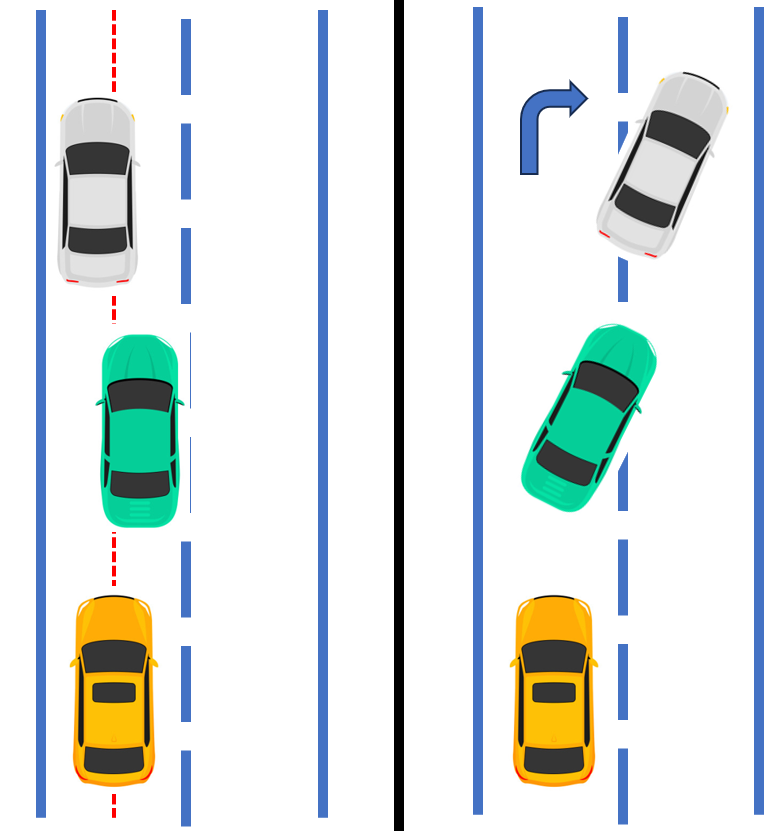
\includegraphics[scale=0.4]{img/2Case_sim.png}
    \caption{Simulation case: "Left image" Perform a platoon try to match the speed and heading angle, "Right image" The platoon try to change the lane, vehicle following behavior.}
    \label{fig:2Case_sim}
\end{figure}

Platoon Control (Left Image):

Vehicles must maintain a safe following distance.
Speed synchronization is crucial to avoid abrupt braking or acceleration.
Heading angles should be matched to ensure stability.
Lane Change Coordination (Right Image):

The lead vehicle initiates the lane change, and the following vehicles must react accordingly.
Communication between vehicles (via V2V communication) is beneficial for smooth transitions.
The vehicle-following behavior ensures that the platoon does not break apart while changing lanes.



\bibliographystyle{IEEEtran}


%=================
\bibliography{biblio}
%=================
\end{document}




% \end{document}
